% Section content template for individual Educative lessons
% This file contains the actual content for a specific section
% Generated from Educative API section content

% Section: Requirements for the Jigsaw Puzzle
% Section ID: 6422319629336576
% Section Slug: requirements-for-the-jigsaw-puzzle
% Generated: 2025-12-14T13:10:21.845090

In this lesson, we'll list the requirements of our jigsaw puzzle problem. This is a crucial step since requirements define the scope of a problem. Getting them right from the interviewer and understanding them well will make the design of the rest of the problem smooth and easy.
\\
We'll use the notational convention to identify each requirement with a unique label ``Rn,'' where ``R'' is short for Requirement and ``n'' is a natural number.

\subsection{Requirement collection}\label{u4-GNiBModuGioypl4XnZ}
\\
For the jigsaw puzzle problem, the requirements are defined below:
\\
\textbf{R1:} Our board will be in the shape of a rectangle.
\\
\textbf{R2:} All pieces will have four sides with an indentation, an extrusion, or a flat edge.
\\
\textbf{R3:} There are four corner pieces, some edge pieces, and the remaining ones are the middle pieces. A corner piece has two flat sides, an edge piece only has one flat side, and a middle piece has no flat edges.

\begin{figure}[htbp]
 \centering
 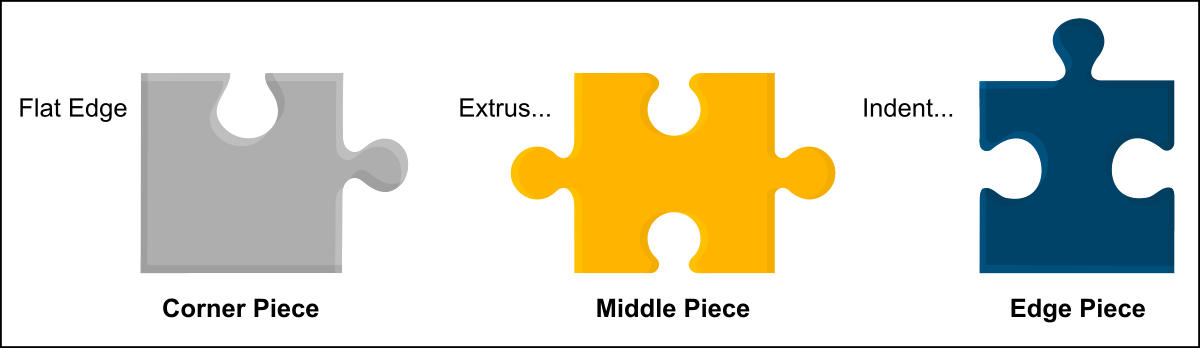
\includegraphics[width=0.5\textwidth]{Images/chapter_24/section_6422319629336576/5039679667961856.png}
 
\end{figure}

\textbf{R4:} All pieces will be unique, so only one piece will fit with one other piece.
\\
\textbf{R5:} Two pieces fit together by the curvature of the indentation on one piece matching up to the curvature of the extrusion on another.

\begin{figure}[htbp]
 \centering
 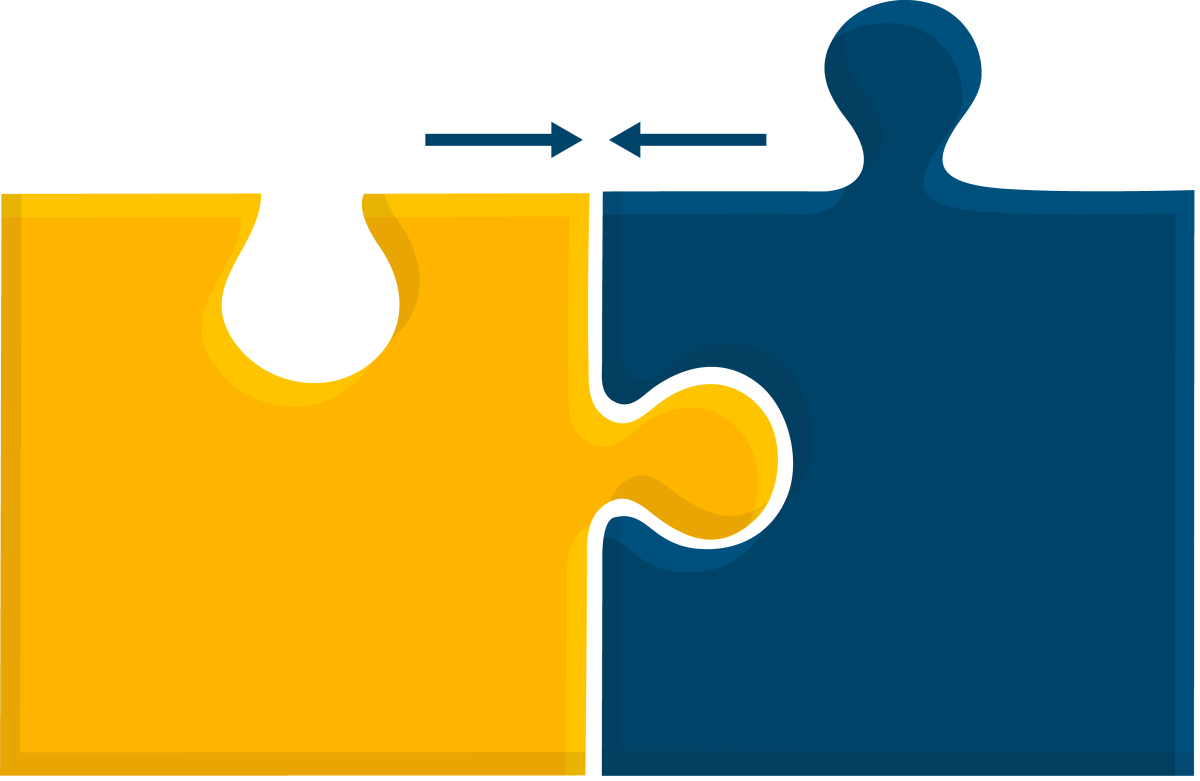
\includegraphics[width=0.15\textwidth]{Images/chapter_24/section_6422319629336576/4948192443760640.png}
 
\end{figure}

We've identified our requirements for the problem, and in the next lesson, we will define the class diagram of our jigsaw puzzle system.

% End of section content